%Created with command:
%"/home/josh/Teaching/trunk/Utilities/makeexam" "Homework 6 - XOR Circuits And Adders" "Please complete the problems below.  As usual you may work together and use other resources including those in the Internet for reference.  However make sure the work that you submit is yours." "../XOR/Assessments/wakerly_6_82.tex" "../XOR/Assessments/wakerly_6_94.tex" "../XOR/Assessments/wakerly_6_96.tex" "../Adders/Assessments/wakerly_6_100.tex"
\documentclass{article}
\usepackage[T1]{fontenc}
\usepackage{arev}
\usepackage{longtable}
\usepackage[hmargin=2cm,vmargin=2cm]{geometry}
\usepackage{graphicx}
\usepackage{listings}
\setlength{\parindent}{0pt}
\title{Homework 6 - XOR Circuits And Adders}
\date{}
\begin{document}
\maketitle
Please complete the problems below.  As usual you may work together and use other resources including those in the Internet for reference.  However make sure the work that you submit is yours. (18 points total)
\begin{longtable}[l]{rp{17cm}}
%file: ../XOR/Assessments/wakerly_6_82.tex
1.&\begin{minipage}[t]{\linewidth}(4 pt) Do problem 6.82 in the text.\\ \\

Solution: \\ \\
The first structure gives a maximum worst-case propagation delay (3 XOR-gate delays), the second gives a minimum(2 XOR-gate delays).  Although it is slower, the first structure allows intermediate parity results to be easily obtained.\\ \\
\begin{center}
  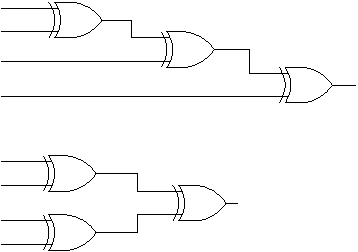
\includegraphics{../XOR/Assessments/Wakerly_6_82} \\
\end{center}
\end{minipage}\\
\medskip
%file: ../XOR/Assessments/wakerly_6_94.tex
2.&\begin{minipage}[t]{\linewidth}(8 pt) Do problem 6.94 in the text.  You do not need to write a test bench, although it may be beneficial to allow you to test your circuit.\\ \\

Solution: \\ \\
\lstset{language=VHDL}
\lstinputlisting{../XOR/Assessments/74x85.vhd}
\end{minipage}\\
\medskip
%file: ../XOR/Assessments/wakerly_6_96.tex
3.&\begin{minipage}[t]{\linewidth}(4 pt) Do problem 6.96 in the text.\\ \\

Solution: \\ \\
\begin{center}
  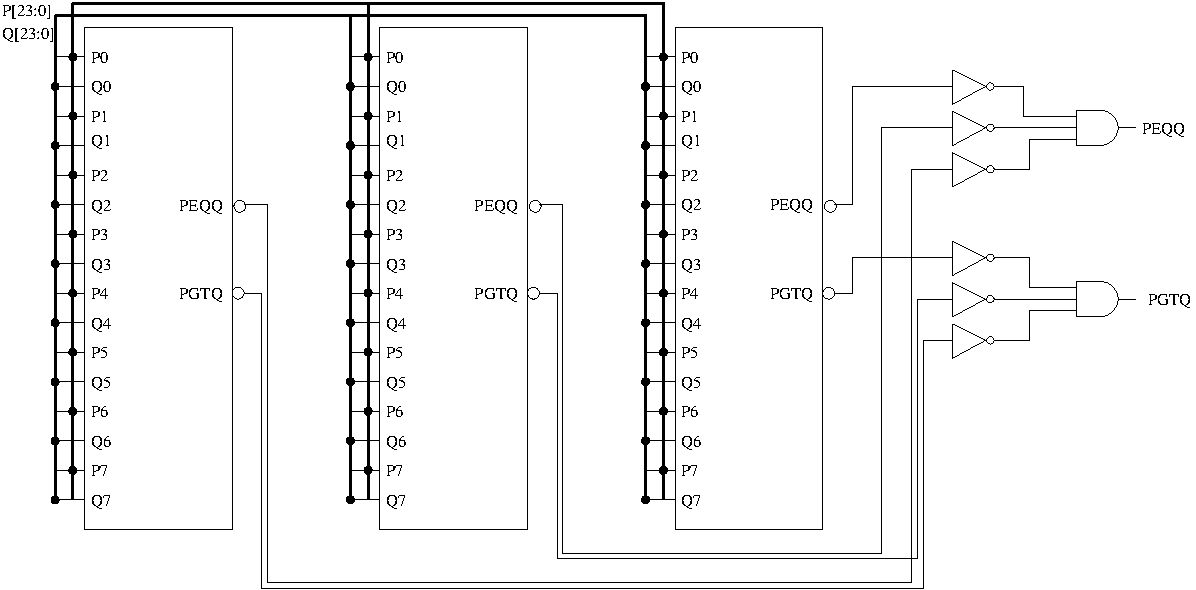
\includegraphics[scale=0.8]{../XOR/Assessments/Wakerly_6_96}
\end{center}
\end{minipage}\\
\medskip
%file: ../Adders/Assessments/wakerly_6_100.tex
4.&\begin{minipage}[t]{\linewidth}(2 pt) Do problem 6.100 in the text.\\ \\

Solution: \\ \\
$S3 = [(A3 \cdot B3)' \cdot (A3 + B3)] \oplus [(A2 + B2) \cdot [(A1 + B1) + (A2 \cdot B2)] \cdot [(A0 + B0) + (A2 \cdot B2) + (A1 + B1)] \cdot [(A2 \cdot B2) + (A1 \cdot B1) + (A0 + B0) + C0]]$
\end{minipage}\\
\medskip
\end{longtable}
\end{document}